\section{Functions, Slope, and Lines} \label{S:0.1.Functions}


\vspace*{-14 pt}
\framebox{\hspace*{3 pt}
\parbox{6.25 in}{\begin{goals}
\item What is a function and what do we mean by its domain and range?
\item What is the slope of a line? What are linear functions and families of linear
    functions?
\item What are difference equations and the delta notation and why are these useful?
\end{goals}} \hspace*{3 pt}}

% \begin{web}
% \item
%     \href{https://www.youtube.com/watch?v=AfoNnJ038zA&list=PL9bIjQJDwfGuXQHuS5Jkmum_CFILoCZX-&index=92}{Video:
%     How to read a math textbook}
% \item
%     \href{https://www.khanacademy.org/math/algebra/solving-linear-equations-and-inequalities}{Khan
%     Playlist: Linear Equations}
% \item \href{https://www.khanacademy.org/math/algebra/algebra-functions}{Khan Playlist:
%     Functions}
% \item \href{https://www.khanacademy.org/math/algebra2/functions_and_graphs}{Khan Playlist:
%     Functions and Graphs}
% \end{web}

\nin \hrulefill



\subsection*{Introduction}
We begin the study of calculus by reminding the reader of several pre-requisite topics.
The study of calculus depends on a thorough understanding of these topics and it is
imperative that the reader become as familiar as possible with these topics.  In the
present section we remind the reader about the concepts of functions, slope, and lines,
but first, there are a few things that you should do to get your self ready to use this
text.

\begin{pa} \label{PA:0.1}
    This is the first Preview Activity in this text.  Your job for this activity is to get
    to know the textbook.
    \ba
    \item Where is the full textbook stored?  Find it and save a copy to your computer.
    \item What chapters of this text are you going to cover this semester.  Have a look at
        your syllabus!
%     \item There are a few appendices in the textbook.  What are they and 
%         where are they?
    \item What are the differences between Preview Activities, Activities, Examples,
        Exercises, Voting Questions, and WeBWork?  Which ones should you do before class,
        which ones will you likely do during class, and which ones should you be doing
        after class?
    \item What materials in this text would you use to prepare for an exam and where do
        you find them?
    \item What should you bring to class every day?
    \ea
\end{pa} \afterpa


\subsection*{Functions}
\begin{definition}
    A {\bf function} $f$ defined on a set $A$, is a rule that assigns to each element $x$ in $A$,
exactly one element, denoted $f(x)$, from a set $B$. 

\noindent The set $A$ is called the {\bf domain} of the function $f$. The {\bf range} of $f$ is the set
of values of $f(x)$
as $x$ takes on all the values of $A$.  Another way to state it is that the range of $f$ is the
set of all $y$ such that $y=f(x)$ for some $x$ in $A$.
\end{definition}

It is easy to give many common examples of functions:
\begin{itemize}
    \item The area of a circle $A$ is a function of the radius of the circle:  $A(r)= \pi r^2$.
    \item The amount $M$ in your savings account is a function of the rate of interest the
        bank pays.
    \item Your miles per gallon in your car depends on many things, e.g. the speed at
        which you drive.  
    \item The pressure on a diver is a function of the depth of the diver under water.
\end{itemize}

Probably the most common method for representing a function is with a graph.  If the
domain of function $f$ is set $A$, then the graph of $f$ is the collection of all ordered
pairs of the form $(x,f(x))$ where $x$ comes from the domain $A$.



\begin{activity}\label{A:0.1.1}
The graph of a function f is shown below. 

\begin{center}
    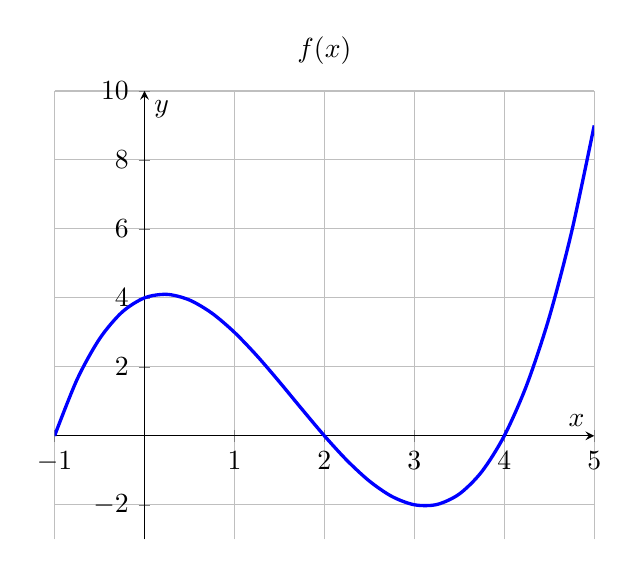
\begin{tikzpicture}
        \begin{axis}[axis lines=center, xmin=-1, xmax=5, ymin=-3, ymax=10, grid,
            xlabel={$x$}, ylabel={$y$}, title={$f(x)$}]
            \addplot[smooth, blue, very thick, domain=-1:5] {0.5*(x+1)*(x-2)*(x-4)};
        \end{axis}
    \end{tikzpicture}
\end{center}

\ba
\item What are the domain and range of $f$?
\item What are  $f(-1)$, $f(1)$, $f(3)$, $f(5)$?
\ea

\end{activity}\aftera


\bex
Find the domain and range of the functions
\[ f(x) = \sin(x), \quad g(x) = \sqrt{x}, \quad \text{and} \quad h(x) =
    \frac{1}{x}. \]
\eex
For $f(x)=\sin(x)$ we recall that the sine function is defined for every possible value of $x$ but
the output is strictly between $y=-1$ and $y=1$.  Therefore, the domain for $f(x) =
\sin(x)$ is $-\infty < x < \infty$ and the range is $-1 \le y \le 1$.  See the left plot
in Figure \ref{f:0.1ex1}.

For $g(x) = \sqrt{x}$ we recall that the square root of a negative number results in an
imaginary number.  In this text we are interested in real-valued output for functions so
we must omit all of the negative numbers from the domain and hence $0 \le x < \infty$.
For the range we recall that the square root of a number will always be a non-negative
number.  As such, the range is $0 \le y < \infty$.  See the middle plot
in Figure \ref{f:0.1ex1}.

For $h(x) = \frac{1}{x}$ we recall that division by zero is mathematically impossible.
That is the only troublesome point in the domain so $-\infty < x < 0$ or $0 < x < \infty$.
A moment's reflection also reveals that it is impossible to get zero out of the function
$h(x)$ but it is possible to get any other number.  Hence $-\infty < y < 0$ or $0 < y <
\infty$. See the right plot in Figure \ref{f:0.1ex1}. 
\afterex

\begin{figure}
    \begin{center}
        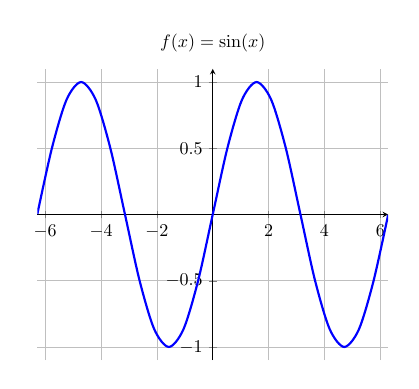
\begin{tikzpicture}[scale=0.65]
            \begin{axis}[axis lines=center, title={$f(x) = \sin(x)$}, domain=-6.28:6.28,
                ymin=-1.1, ymax = 1.1, grid]
                \addplot[smooth, very thick, blue] {sin(deg(x))};
            \end{axis}
        \end{tikzpicture}
        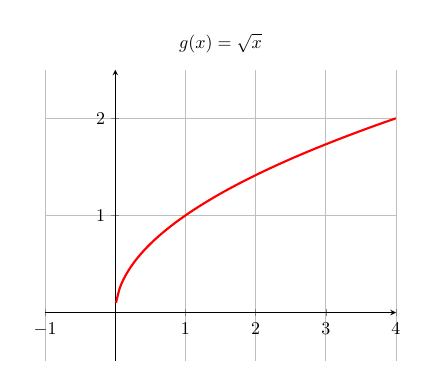
\begin{tikzpicture}[scale=0.65]
            \begin{axis}[axis lines=center, title={$g(x) = \sqrt{x}$}, domain=-1:4,
                ymin=-0.5, ymax = 2.5, xmin=-1, grid]
                \addplot[smooth, very thick, red, samples=100] {sqrt(x)};
            \end{axis}
        \end{tikzpicture}
        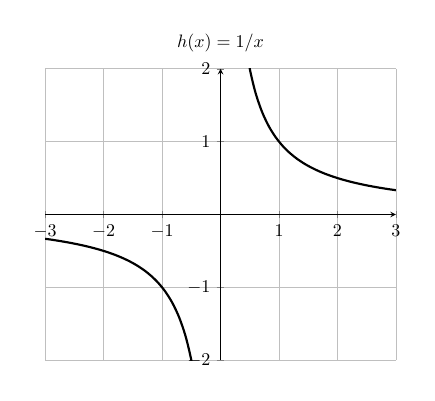
\begin{tikzpicture}[scale=0.65]
            \begin{axis}[axis lines=center, title={$h(x) = 1/x$},
                ymin=-2, ymax = 2, grid]
                \addplot[smooth, very thick, domain=-3:-0.1, black] {1/x};
                \addplot[smooth, very thick, domain=0.1:3, black] {1/x};
            \end{axis}
        \end{tikzpicture}
    \end{center}
    \caption{Graphs of the function $f(x) = \sin(x)$, $g(x) = \sqrt{x}$, and $h(x) =
    \frac{1}{x}$.}
    \label{f:0.1ex1}
\end{figure}

\subsection*{Slope and Linear Functions}
In Calculus we are often interested in writing the equation for a linear function.  As
such, we should review the features of linear functions.  Every linear function is
characterized by a constant rate of change; the slope.  The slope of a linear function is
a measure of the ``steepness'' of the line.  We use the symbols $\Delta x$,
$\Delta y$ which
mean respectively the ``change in $x$'' and the ``change in $y$''.  
\begin{definition}
    The {\bf slope}, $m$ of a (non-vertical) linear function $f$ which passes through any
    two points $(x_1,y_1)$, $(x_2,y_2)$ can be found using the formula
    \[ m = \frac{\Delta y}{\Delta x} = \frac{y_2 - y_1}{x_2 - x_1} =
    \frac{f(x_2)-f(x_1)}{x_2-x_1} = \frac{\text{Rise}}{\text{Run}} \]
\end{definition}

\begin{minipage}{0.4\columnwidth}
    Recall that
\begin{itemize}
    \item if the line rises from left to right then the slope is positive,
    \item if the line falls from left to right then the slope is negative,
    \item if the line is horizontal then the slope is zero, and
    \item if the line is vertical then the slope is undefined.
\end{itemize}
\end{minipage}
\begin{minipage}{0.5\columnwidth}
    \begin{center}
        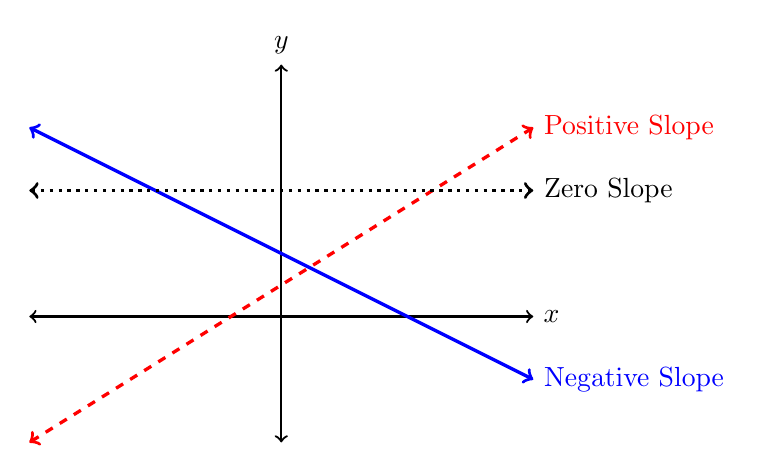
\begin{tikzpicture}[scale=0.8]
            \draw[<->, thick] (-4,0) -- (4,0) node[anchor=west]{$x$};
            \draw[<->, thick] (0,-2) -- (0,4) node[anchor=south]{$y$};
            \draw[<->, very thick, blue] (-4,3) -- (4,-1) node[anchor=west]{Negative
            Slope};
            \draw[<->, very thick, color=red, dashed] (-4,-2) -- (4,3)
            node[anchor=west]{Positive Slope};
            \draw[<->, very thick, color=black, dotted] (-4,2) -- (4,2)
            node[anchor=west]{Zero Slope};
        \end{tikzpicture}
    \end{center}
\end{minipage}\bigskip

Depending on the information given there are several convenient forms of the equation of a
line.  Given the definition of the slope
\[ m = \frac{y_2 - y_1}{x_2 - x_1} \]
and letting $(x,y) = (x_2,y_2)$ be any arbitrary point we get the point-slope form of a
linear function.
\begin{definition}
If the linear function $f$ has slope $m$ and passes through the
point $(x_1,y_1)$, then the {\bf point-slope form of the equation of a line} is given by: 
\[ y-y_1=m(x- x_1).  \]
\end{definition}

An alternate form of a linear function which is probably very familiar to most readers is
the slope-intercept form of a line.
\begin{definition}
If the linear function $f$ has slope $m$ and $y$-intercept $b$, then the
{\bf slope-intercept form of the equation of a line} is given by: 
\[ y=mx + b.  \]
\end{definition}
In a calculus class the point-slope form is often the most useful. The
symbols and geometry used in each of the above definitions are shown in Figure
\ref{fig:0.1.linear_fn}.

\begin{figure}[ht!]
    \centering
    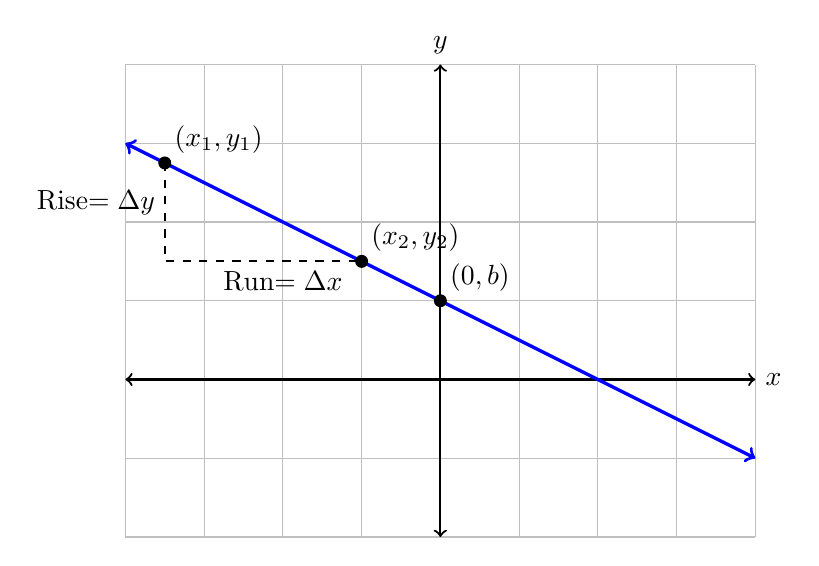
\begin{tikzpicture}
        \draw[color=gray!50] (-4,-2) grid (4,4);
        \draw[<->, thick] (-4,0) -- (4,0) node[anchor=west]{$x$};
        \draw[<->, thick] (0,-2) -- (0,4) node[anchor=south]{$y$};
        \draw[<->, very thick, blue] (-4,3) -- (4,-1);
        \draw[color=black, fill=black] (-3.5,2.75) circle(0.075cm) node[anchor=south
        west]{$(x_1,y_1)$};
        \draw[color=black, fill=black] (-1,1.5) circle(0.075cm) node[anchor=south
        west]{$(x_2,y_2)$};
        \draw[color=black, fill=black] (0,1) circle(0.075cm) node[anchor=south
        west]{$(0,b)$};
        \draw[thick, dashed] (-3.5,2.75) -- (-3.5,1.5) -- (-1,1.5);
        \draw (-3.5,2.25) node[anchor=east]{Rise$=\Delta y$};
        \draw (-2,1.5) node[anchor=north]{Run$=\Delta x$};
    \end{tikzpicture}
    \caption{Anatomy of a linear function.}
    \label{fig:0.1.linear_fn}
\end{figure}


\begin{activity}\label{A:0.1.2}
Find the equation of the line with the given information.
\ba
\item The line goes through the points $(-2,5)$ and $(10,-1)$.
\item The slope of the line is $3/5$ and it goes through the point $(2,3)$.
\item The $y$-intercept of the line is $(0,-1)$ and the slope is $-2/3$.
\ea

\end{activity}
\begin{smallhint}
   \ba
        \item Recall that $m = \frac{\Delta y}{\Delta x}$ and use the point slope form of
            the line.
        \item You are given a slope and a point.  Which form of the line should you use?
        \item You are given a slope and the $y$ intercept.  Which form of the line should
            you use?
   \ea
\end{smallhint}
\begin{bighint}
   \ba
        \item The slope is $m = \frac{\Delta y}{\Delta x} = \frac{5-(-1)}{(-2)-10} =
            \frac{6}{-12} = -\frac{1}{2}$.  Now use the point-slope form of the line.
        \item The point-slope form of the line is best here.
        \item The slope-intercept form of the line is best here.
   \ea
\end{bighint}
\begin{activitySolution}
   \ba
        \item The slope is $m = \frac{\Delta y}{\Delta x} = \frac{5-(-1)}{(-2)-10} =
            \frac{6}{-12} = -\frac{1}{2}$.  Hence,
            \[ y - 5 = -\frac{1}{2} \left( x-(-2) \right) \]
            which can be rewritten as
            \[ y = -\frac{1}{2} \left( x+2 \right) + 5. \]
        \item Using the point-slope form of the line we get
            \[ y - 3 = \frac{3}{5} \left( x-2 \right) \]
            which can be rearranged to 
            \[ y = \frac{3}{5} \left( x-2 \right) + 3. \]
        \item Using the slope-intercept form of the line we get
            \[ y = -\frac{2}{3} x - 1. \]
   \ea
\end{activitySolution}
\aftera


\bex
Write the equation of the line going through the points $(5,7)$ and $(-3,2)$.
\eex
First we calculate the slope 
\[ m = \frac{\Delta y}{\Delta x} = \frac{7 - 2}{5-(-3)} = \frac{5}{8}. \]
Since we have two points and neither is the $y$ intercept of the linear function we choose
to use the point-slope form of the line.  Letting $(x_1,y_1) = (5,7)$ we see that
\[ y - 7 = \frac{5}{8} \left( x-5 \right) \]
is one form of the linear function.  
It is often conventient to solve for $y$ giving us
\[ y = \frac{5}{8} \left( x-5 \right) + 7. \]
Notice that we do not necessarily need to simplify all the way to the slope-intercept form
of the line.  
\afterex

\subsection*{Linear Functions From Data}
A feature of every linear function is that the slope is the same no matter where you are
on the line.  When given a table of data that you suspect might represent a linear
function the slope manifests itself as a constant common difference between successive
$y$-values.  

\bex
Consider the data in the table below.
\begin{center}
    \begin{tabular}[h!]{|c||c|c|c|c|c|}
        \hline
        $x$ & 5 & 6 & 7 & 8 & 9 \\ \hline
        $y$ & 12.2 & 17.5 & 22.8 & 28.1 & 33.4 \\ \hline
    \end{tabular}
\end{center}
Demonstrate that this data is linear and write an equation that fits the data.
\eex
The common differences can be found for each successive $y$-values
\begin{center}
    \begin{tabular}[h!]{|c||c|c|c|c|c|}
        \hline
        $x$ & 5 & 6 & 7 & 8 & 9 \\ \hline
        $y$ & 12.2 & 17.5 & 22.8 & 28.1 & 33.4 \\ \hline
        Common Difference & $\frac{17.5-12.2}{6-5} = 5.3$ & $\frac{22.8-17.5}{7-6} = 5.3$
        & $\frac{28.1-22.8}{8-7} = 5.3$ & $\frac{33.4-28.1}{9-8}=5.3$ & - \\ \hline
    \end{tabular}
\end{center}
The successive differences are clearly the same throughout the data set and the slope for
this data set is $m=5.3$.  Picking any convenient point, say $(5,12.2)$, then allows us to write the
equation of the line as 
\[ y - 12.2 = 5.3(x-5). \]
This could be simplified to point-slope form, but there is typically no need for this
algebraic simplification.
\afterex


\begin{activity}\label{A:0.1.3}
A simulation shows lifetime peptic ulcer rates per 100 population for different
family incomes as given in the following table.

\begin{minipage}{0.3\columnwidth}
    \begin{center}
    \begin{tabular}{|c|c|}
        \hline
        Income  & Ulcer Rate\\
        \hline \hline
        \$4000  & 14.1\\
        \$8000  & 13.4\\
        \$12000 &12.5\\
        \$16000 &12\\
        \$20000 &12.4\\
        \$24000 &11.6\\
        \$28000 &10.8\\
        \$32000 &10.3\\
        \$36000 &10.4\\
        \$40000 & 9.6\\
        \$44000 & 9.2\\
        \$48000 & 8.8\\
        \$52000 & 8.5\\
        \$56000 & 8.4\\
        \$60000 & 8.2\\ \hline
    \end{tabular}
\end{center}
\end{minipage}
\begin{minipage}{0.3\columnwidth}
    \begin{center}
        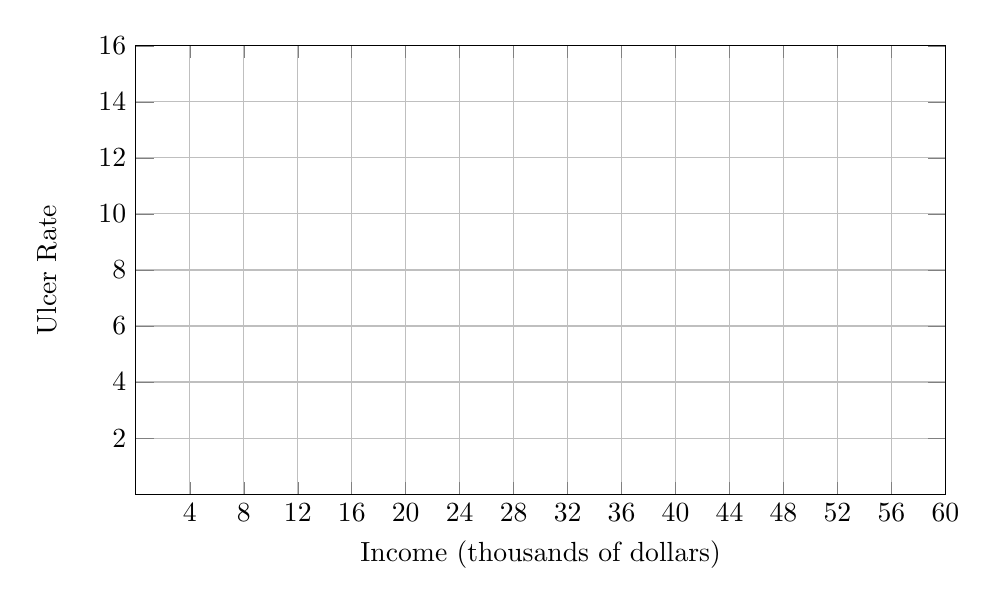
\begin{tikzpicture}
            \begin{axis}[xmin=0, xmax=60, ymin=0, ymax=16, xlabel={Income (thousands of
                dollars)}, ylabel={Ulcer Rate}, grid,
            xtick={4,8,12,16,20,24,28,32,36,40,44,48,52,56,60}, xscale=1.5,
        ytick={2,4,6,8,10,12,14,16}]
                \addplot[smooth] {0*x};
            \end{axis}
        \end{tikzpicture}
    \end{center}
\end{minipage}

This data does not represent a straight line, but it is close.
\ba 
\item Just by doing simple arithmetic, how can you tell the function is not a straight
    line?

\item Make a scatter plot of the data.  Do you think a linear model can be a good
    approximation?  Why or why not?

\item Use just the first and the last data points, what is the equation of the straight
    line that these two points determine?  Graph this equation.

\item Using the model in part (c), estimate the ulcer rate for an income of \$26000.

\item Using the model in part (c), how likely is someone with an income of \$100,000 will
    suffer from peptic ulcers?  Note your answer will be a percent and remember that the
    ulcer rate is given per 100 people of population.

\item Do you think it would be reasonable to apply this model to a person with an income
    of \$200,000?  Why or why not?
\ea
\end{activity}
\begin{smallhint}
   \ba
        \item Recall what we know about slope on a linear function.
        \item The data do not fall on one line, but are they close?
        \item It might be best to find slope first
        \item Once you have the linear function you can use it to make predictions.
        \item 
        \item
   \ea
\end{smallhint}
\begin{bighint}
   \ba
        \item
        \item
        \item
        \item
        \item
        \item
   \ea
\end{bighint}
\begin{activitySolution}
   \ba
        \item 
        \item
        \item
        \item
        \item
        \item
   \ea
\end{activitySolution}
\aftera



\bex
The Old Farmer's Almanac tells us that you can tell the temperature by counting the chirps
of a cricket.  It is a linear function $T=f(C)$ given by $T$ (in degrees Fahrenheit)=\# of
chirps in 15 seconds $+40$.  We can approximate this with the formula 
\[ T =  \frac{C}{4} + 40 \]
where $C$ is the number of chirps/minute and $T$ is in $^\circ F$.
\ba
    \item If the chirp rate is 120 chirps/minute, what is the temperature?
    \item Suppose that crickets will not chirp if the temperature is below $56^\circ F$.
        We can also suppose that crickets will not chirp above $136^\circ F$ since that is
        the highest temperature ever recorded at a weather station.  With these
        parameters, what is the domain of this function?
\ea
\eex
\ba
    \item If $C = 120$ chirps/minute, substitute this into the function $T(C)$ to obtain
        \[ T(120) = \frac{120}{4} + 40 = 30 + 40 = 70^\circ F. \]
    \item To find the domain we need to find the appropriate values of $C$ for the $T(C)$
        function.  Solve $56=C/4+40$ and get $C = 64$.  Solve $136=C/4+40$ and get $C =
        384$.  So the domain of $T(C)$ is $64 \le \text{chirps/minute} \le 384$ or, in
        interval notation, $[64, 136]$. 

\ea
\afterex


\subsection*{Families of Linear Functions}
We noted above that a linear function has the form  $y=f(x)=mx+b$, where $m$ is the slope of
the line, and $b$ is the $y$-intercept.  Since $m$ and $b$ can take on various values, taken
together, they represent a family of functions.  For example, we could fix $b = 2$, and then
draw the graphs of $f(x)=mx+2$ for various values of $m$; for example, $m = -1, -2, 2, 1$.
Doing so would give the functions in the family $f(x)=mx+2$ shown in the left image of Figure
\ref{fig:0.1.fam1}.

Similarly, we could set $m$ to be $2$ and let $b$ take on the values $b=-1, 1, 4, -6$ and
we would get
some examples from the family of functions for $y=f(x)=2x+b$ shown in the right image of Figure
\ref{fig:0.1.fam1}.


From the right image in Figure \ref{fig:0.1.fam1} it should be clear to the reader that
parallel lines have the same slope.  What can you say about the slopes of perpendicular
lines?  Here is the result that we state without proof.
\begin{theorem}\label{thm:test}
If line $\ell_1$ has slope $m_1$ and line $\ell_2$ has slope $m_2$, then 
    \begin{itemize}
        \item lines $\ell_1$ and $\ell_2$ are parallel if the slopes are the same: $m_1 = m_2$,
            and
        \item lines $\ell_1$ and $\ell_2$ are perpendicular if the slopes are opposite
            reciprocals: $m_2 = -\frac{1}{m_1}$.
    \end{itemize}
\end{theorem}

\def\scl{0.8}
\begin{figure}[ht]
    \centering
    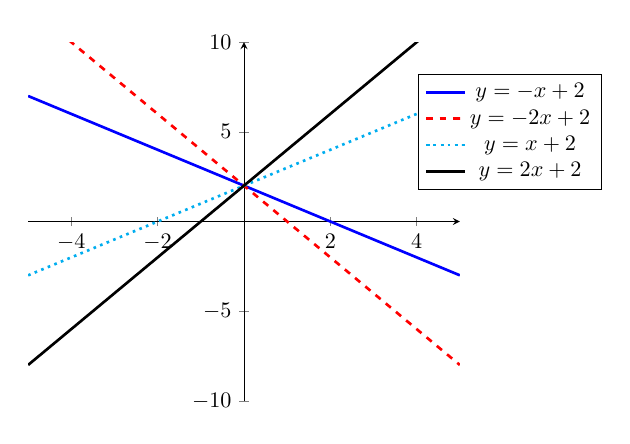
\begin{tikzpicture}[scale=\scl]
        \begin{axis}[axis lines=center, xmin=-5, xmax=5, ymin=-10, ymax=10,
            legend style={ at={(axis cs:4.03,5)}, anchor=west }]
            \addplot[smooth, very thick, color=blue] {-1*x+2};
            \addlegendentry{$y=-x+2$};
            \addplot[smooth, very thick, color=red, dashed] {-2*x+2};
            \addlegendentry{$y=-2x+2$};
            \addplot[smooth, very thick, color=cyan, dotted] {1*x+2};
            \addlegendentry{$y=x+2$};
            \addplot[smooth, very thick, color=black] {2*x+2};
            \addlegendentry{$y=2x+2$};
        \end{axis}
    \end{tikzpicture}
    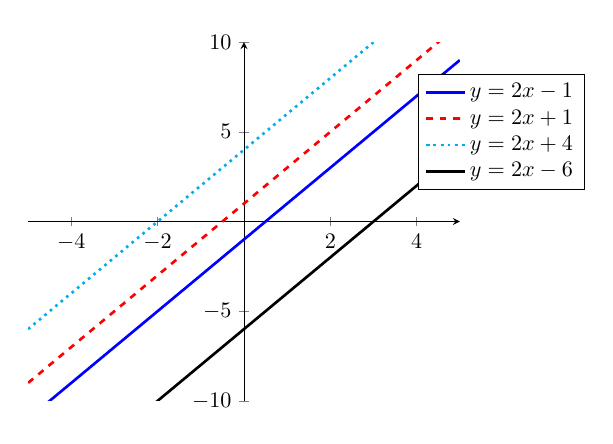
\begin{tikzpicture}[scale=\scl]
        \begin{axis}[axis lines=center, xmin=-5, xmax=5, ymin=-10, ymax=10,
            legend style={ at={(axis cs:4.03,5)}, anchor=west }]
            \addplot[smooth, very thick, color=blue] {2*x-1};
            \addlegendentry{$y=2x-1$};
            \addplot[smooth, very thick, color=red, dashed] {2*x+1};
            \addlegendentry{$y=2x+1$};
            \addplot[smooth, very thick, color=cyan, dotted] {2*x+4};
            \addlegendentry{$y=2x+4$};
            \addplot[smooth, very thick, color=black] {2*x-6};
            \addlegendentry{$y=2x-6$};
        \end{axis}
    \end{tikzpicture}
    \caption{Several members of the family of linear functions $f(x) = mx+2$ (left) and
    the family $f(x) = 2x+b$ (right).}
    \label{fig:0.1.fam1}
\end{figure}

\begin{activity}\label{A:0.1.4}
Write the equation of the line with the given information.
\ba
\item Write the equation of a line parallel to the line $y=\frac{1}{2}x+3$ passing through
    the point $(3,4)$.
\item Write the equation of a line perpendicular to the line $y=\frac{1}{2}x + 3$ passing
    through the point $(3,4)$.
\item Write the equation of a line with $y$-intercept $(0,-3)$ that is perpendicular to
    the line $y=-3x-1$.
\ea
\end{activity}
\begin{smallhint}
    \ba
        \item What is the slope of the line that you're given and which form of a linear
            function would be most convenient?
        \item What is the slope of the line that you're given and which form of a linear
            function would be most convenient?
        \item You are given the $y$-intercept.  Why is that a special case?
    \ea
\end{smallhint}
\begin{bighint}
    \ba
        \item The slope should be the same since the lines are parallel.
        \item The slope should be the opposite reciprocal since the lines are
            perpendicular.
        \item The slope should be the opposite reciprocal since the lines are
            perpendicular.
    \ea
\end{bighint}
\begin{activitySolution}
    \ba
        \item The slope is $m = \frac{1}{2}$ and you have a point so use the point-slope
            form of the line to get
            \[ y - 4 = \frac{1}{2} \left( x-3 \right). \]
            Solving for $y$ we get 
            \[ y = \frac{1}{2} \left( x-3 \right) + 4. \]
        \item The slope is $m = -2$ and we have a point so use the point-slope form of the
            line to get
            \[ y - 4 = -2 (x-3). \]
            Solving for $y$ we get 
            \[ y = -2(x-3) + 4. \]
        \item The slope is $m = \frac{1}{3}$ and since we have the $y$-intercept we know
            that the slope-intercept for the line is the proper choice.  Hence,
            \[ y = \frac{1}{3} x - 3. \]
    \ea
\end{activitySolution}



\aftera



% \subsection*{Equations, Functions, and Expressions}
% To conclude this first section we define three commonly misused mathematical terms.
% \begin{definition}
%     A {\bf mathematical expression} is a combination of numbers, variables, and operations
%     (addition, subtraction, multiplication, roots, etc).  Several examples are:
%     \begin{itemize}
%         \item $2x+3$
%         \item $\sqrt{a^2 + b^2}$
%         \item $\pi r^2$
%     \end{itemize}
% \end{definition}
% 
% \begin{definition}
%     An {\bf equation} is a mathematical statement containing an equal sign where the left
%     and right-hand sides of the equal sign are expressions in the same variable.  Examples
%     are:
%     \begin{itemize}
%         \item $3=5x-2$
%         \item $x^2-2x+5=9$
%         \item $\sqrt{3x-2} = 19$
%     \end{itemize}
% \end{definition}
% 
% \begin{definition}
%     A {\bf function} (as defined before) is a rule that associates a value $x$ in the
%     domain to a value $y$ in the range.  Examples include:
%     \begin{itemize}
%         \item $y=x^2+3$
%         \item $f(x) = 3x-4$
%         \item $f(y) = \sqrt{3y-2}$
%     \end{itemize}
% \end{definition}
% 
% It is easy for students to confuse the meanings of these three definitions, so here are
% some helpful tips:
% \begin{itemize}
%     \item If there is no equal sign then it is an expression.
%     \item It makes sense to substitute a value into an expression, but saying that you're
%         going to ``solve'' an expression is meaningless.
%     \item If it is an equation then it is meaningful to ``solve'' the equation.  It is NOT
%         meaningful to say that you are going to ``solve'' a function or expression.
%     \item A function defines a rule that associates two variables.
%     \item A function has an associated graph whereas expressions and equations do not.
% \end{itemize}
% 
% \begin{activity}\label{A:0.1.5}
    Classify each of the following as an expression, equation, or a function.  For each
    function, classify it as either linear or non-linear.  Finally, for each linear
    function find the slope and $y$-intercept.
    \ba
    \item $y=6y-3$
    \item $y=6x-3$
    \item $6x-3$
    \item $-4y+2x+8=0$
    \item $12x=6y+4$
    \item $12x=6y^2+4$
    \item $\sqrt{x+2}$
    \item $y=\sqrt{x+2}$
    \item $x=\sqrt{x+2}$
    \item $x^2+2x-3$
    \item $x+2x-3=9$
    \ea

\end{activity}\aftera

% 
% % more activites

\begin{summary}
\item A function assigns one $y$ value to each $x$ value.
\item The slope of a linear function can be written as 
    \[ m = \frac{\text{Rise}}{\text{Run}} = \frac{y_2 - y_1}{x_2 - x_2} \]
\item A linear function can be written in the forms
    \[ y = mx + b \quad \text{or} \quad y-y_1 = m(x-x_1) \]
\item When examining linear data, the differences between successive $y$-values reveals
    the slope.
\end{summary}

\nin \hrulefill

% exercises go here
\begin{exercises} 

\item (modified from NCTM Illuminations) The table below displays data that relate the number of oil changes per year and the
    cost of engine repairs.  To predict the cost of repairs from the number of oil
    changes, use the number of oil changes as the $x$ variable and the engine repair cost
    as the $y$ variable.  
    \begin{center}
        \begin{tabular}[h!]{|c|c|}
            \hline
            Oil Changes Per Year & Cost of Repairs (\$) \\ \hline \hline
            3 & 300 \\ 
            5 & 300 \\ 
            2 & 500 \\
            3 & 400 \\ 
            1 & 700 \\
            4 & 400 \\
            6 & 100 \\
            4 & 250 \\ 
            3 & 450 \\
            2 & 650 \\
            0 & 600 \\ 
            10 & 0 \\
            7 & 150 \\ \hline
        \end{tabular}
    \end{center}

    \ba
    \item Using graph paper make a plot of the data on appropriate axes.
    \item Do the data appear linear?  Why or why not?
    \item Pick two representative points from the data and use them to write the
        equation of a line that {\it fits} the data.  Plot your line on top of your data
        and discuss how well your line fits the
        data.   (This may take a few attempts.)
    \item Despite how well your data fit a linear model, it is not entirely sensible to
        use a linear model for this data.  Why?
    \ea
    
\begin{exerciseSolution}
\end{exerciseSolution}


\end{exercises}
\afterexercises







\clearpage

